\subsection{Create lines}
\begin{enumerate}
	\setlength\itemsep{2mm}
	
	\item In the geometry toolbar click on either:  
		\begin{itemize}
		\setlength\itemsep{2mm}
		\item 
\includegraphics{createLine.png}   Create line 
		
		\item 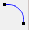
\includegraphics{createArc.png}  Create arc 
		
		\item 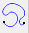
\includegraphics{createNurbsLine.png} Create nurbs line 
		\end{itemize}
	\item Create the line by clicking on the domain or fill in the coordinates in the command line below. When the line is finished, press ESC. 
	
	\item 
\includegraphics{movePoint.png} In order to change the location of the line, press the “move a point” button on the left toolbar.  In the domain click on a point of the line to select it. Click somewhere else in the domain or fill in the new coordinates to move the point to that location. 
	
	\item Lines always have to be connected to other lines by points. In order to add extra points on an existing line, there are the following options
	
	\begin{itemize}
	\setlength\itemsep{2mm}
		\item 
\includegraphics{divideLineNrDiv.png}   Divide a line in a number of divisions 
	
		\item 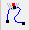
\includegraphics{divideLineNearPoint.png}  Divide a line near a point
	
		\item 
\includegraphics{divideLineAtIntersectLine.png} Divide a line on intersecting lines  
	\end{itemize}

	\end{enumerate}

\subsection{Create surfaces}

\begin{enumerate}
	\setlength\itemsep{2mm}
	
	\item To create a surface there are 2 options:
	\begin{itemize}
		\setlength\itemsep{2mm}
		\item 
\includegraphics{createObject.png}   click on create object and choose either: \textbf{Rectangle}, \textbf{Polygon} or \textbf{Circle}. And draw the surface in the geometry view, or fill in the coordinates in the command line.
		
		\item   Create lines as described before. Connect the lines until a closed shape is formed. Click on "Create NURBS surface" 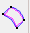
\includegraphics{createNurbsSurface.png} and select the lines in the geometry view which should form the boundary of your surface. Press ESC to finish. \\\\
		\textit{	(Note that lines have to be connected through points, when one line  finishes halfway on another line, this is not considered as a closed surface. Another point has to be added to the second line to form a closed surface.) }
	\end{itemize}

	\item In order to divide a surface into multiple surfaces click on either of the following buttons on the Geometry toolbar:
		\begin{itemize}
		\setlength\itemsep{2mm}
		\item 
\includegraphics{divideSurfaceInNParts.png}  Divide the surface in n even parts
		\item 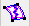
\includegraphics{splitSurfaceFromPathOfLines.png} Divide the surface through a path of lines
		
		\item 
\includegraphics{intersectSurfaceWithLines.png} Intersect the surface through lines
		
		\item 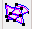
\includegraphics{intersectMultipleSurfaces.png} Intersect the surface with other surfaces
		
	\end{itemize}

\end{enumerate}

\subsection{Create volumes}

\begin{enumerate}
	\setlength\itemsep{2mm}
	\item In order to create volumes there are multiple options:
		\begin{itemize}
		\setlength\itemsep{2mm}
		
		\item  
\includegraphics{createObject.png}   click on create object and choose either: \textbf{Sphere}, \textbf{Cylinder}, \textbf{Cone}, \textbf{Prism} or \textbf{Thorus}. And draw the volume in the geometry view, or fill in the coordinates in the command line.
		
		\item In this option, a volume is created by stretching a surface in the 3rd dimension. 
		\begin{enumerate}
			\setlength\itemsep{2mm}
			\item In the top menu bar go to: Utilities -> Copy… 
			\item In the Copy window set entities type to “Surfaces”
			\item In the Copy window set Transformation to “Translation”
			\item In the Copy window set the first and second point (there should be a difference between the z values in order to create a volume)
			\item In the Copy window set Do extrude to “Volumes”  and unselect “Create contacts” in order to create a volume with more than 1 element in the Z-direction
		\end{enumerate}
		
		\item An other option is to create a volume from connected surfaces. Create surfaces and connect them until a closed 3 dimensional shape is formed. Click on "create volume" 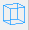
\includegraphics{createVolume.png} and select the surfaces in the geometry view which should form the boundaries of the volume. Press ESC to finish.
		
		\end{itemize}
	
	
\end{enumerate}